% Compile with: pdflatex ADVANCED_PROJECT_REPORT.tex
\documentclass[10pt,twocolumn,a4paper]{article}

\usepackage[a4paper,margin=0.65in]{geometry}
\usepackage[T1]{fontenc}
\usepackage[utf8]{inputenc}
\usepackage{lmodern}
\usepackage{microtype}
\usepackage{amsmath}
\usepackage{amssymb}
\usepackage{array}
\usepackage{booktabs}
\usepackage{enumitem}
\usepackage{graphicx}
\usepackage{hyperref}
\usepackage{caption}
\usepackage{subcaption}
\usepackage{tikz}
\usepackage{pgfplots}
\usepackage{titlesec}
\usepackage{xcolor}

\usetikzlibrary{arrows.meta,positioning,calc,fit,backgrounds,shapes.geometric}
\pgfplotsset{compat=1.18}
\setlength{\columnsep}{0.22in}
\setlength{\parindent}{0pt}
\setlength{\parskip}{3pt}
\setlist[itemize]{leftmargin=*, itemsep=2pt, topsep=2pt}
\setlist[enumerate]{leftmargin=*, itemsep=2pt, topsep=2pt}

\definecolor{brandblue}{HTML}{1D4ED8}
\definecolor{brandgreen}{HTML}{047857}
\definecolor{brandorange}{HTML}{C2410C}
\definecolor{brandpurple}{HTML}{6D28D9}
\definecolor{softblue}{HTML}{EFF6FF}
\definecolor{softgreen}{HTML}{ECFDF5}
\definecolor{softorange}{HTML}{FFF7ED}
\definecolor{softpurple}{HTML}{F5F3FF}
\definecolor{linegray}{HTML}{475569}

\hypersetup{
  colorlinks=true,
  linkcolor=brandblue,
  urlcolor=brandblue,
  citecolor=brandblue,
  pdftitle={Brilliant Minds Hub Advanced Project Report},
  pdfauthor={OpenAI Codex},
}

\titleformat{\section}{\large\bfseries\color{brandblue}}{\thesection.}{0.45em}{}
\titleformat{\subsection}{\normalsize\bfseries\color{brandgreen}}{\thesubsection}{0.4em}{}

\newcommand{\tech}[1]{\texttt{#1}}
\newcommand{\project}{Brilliant Minds Hub}

\tikzset{
  flow/.style={
    rectangle,
    rounded corners=4pt,
    draw=brandblue!70,
    fill=softblue,
    thick,
    align=center,
    minimum height=0.82cm,
    minimum width=2.55cm,
    font=\footnotesize
  },
  store/.style={
    rectangle,
    rounded corners=4pt,
    draw=brandgreen!70!black,
    fill=softgreen,
    thick,
    align=center,
    minimum height=0.82cm,
    minimum width=2.55cm,
    font=\footnotesize
  },
  decision/.style={
    diamond,
    draw=brandorange!80!black,
    fill=softorange,
    thick,
    align=center,
    aspect=1.9,
    inner sep=1.5pt,
    font=\footnotesize
  },
  insight/.style={
    rectangle,
    rounded corners=4pt,
    draw=brandpurple!80,
    fill=softpurple,
    thick,
    align=center,
    minimum height=0.82cm,
    minimum width=2.55cm,
    font=\footnotesize
  },
  line/.style={-{Latex[length=2mm]}, thick, draw=linegray},
  group/.style={draw=linegray!60, dashed, rounded corners=6pt, inner sep=5pt}
}

\title{\vspace{-0.9cm}\textbf{\project}\\Advanced Two-Column Technical Project Report}
\author{Prepared from the repository state dated 2026-04-14}
\date{}

\begin{document}
\maketitle
\thispagestyle{empty}

\begin{abstract}
\project{} is a classroom-aware GATE DA preparation platform with two tightly connected experiences: a student workspace for subject practice, adaptive testing, AI-guided coaching, history review, and assignments, and a teacher command center for course creation, assignment publishing, learner monitoring, intervention planning, and analytics. The system combines role-based product design, Supabase-backed multi-schema data modeling, graph-driven recommendation logic, remediation-aware adaptive sequencing, telemetry via activity events, hybrid AI coaching, and score prediction. This report summarizes the full system architecture, recommendation engines, analytics layer, data flow, and research assets in a formal two-column paper format with embedded visualizations.
\end{abstract}

\section{Executive Overview}
\project{} is not only a mock-test portal. It is an educational intelligence system designed to answer four core questions:

\begin{itemize}
  \item What should the student solve next?
  \item What should the student revise next?
  \item Which learners or courses need teacher intervention?
  \item How can the full learning path be measured, reviewed, and explained?
\end{itemize}

The platform addresses these questions through multiple recommendation systems operating together:

\begin{itemize}
  \item a graph-based adaptive next-question engine
  \item a remediation and retry engine for missed questions
  \item a timing-aware practice review and ELO adjustment system
  \item a hybrid AI coach with deterministic fallback and optional LLM integration
  \item teacher-facing class insight and intervention recommendation logic
  \item a GATE score prediction model based on accuracy, ELO, consistency, and completion
\end{itemize}

\section{Platform Scope}
\subsection{Student Workspace}
\begin{itemize}
  \item authentication, profile creation, theme, and settings
  \item join-code based classroom enrollment
  \item subject and topic navigation with notes
  \item full-paper mock mode, topic-wise tests, and adaptive practice
  \item assignment attempts and score review
  \item dashboard analytics and history review
  \item AI coaching and study guidance
\end{itemize}

\subsection{Teacher Command Center}
\begin{itemize}
  \item teacher workspace provisioning
  \item course creation with unique join codes
  \item enrollment and roster tracking
  \item assignment authoring and publication
  \item submission monitoring
  \item teacher dashboard, course analytics, and student profile inspection
  \item intervention support through weak-topic and risk analysis
\end{itemize}

\section{Technology Stack}
\begin{table}[h]
\centering
\footnotesize
\begin{tabular}{>{\raggedright\arraybackslash}p{0.22\columnwidth} >{\raggedright\arraybackslash}p{0.68\columnwidth}}
\toprule
Layer & Technologies \\
\midrule
Frontend & React 18, TypeScript, Vite \\
UI & Tailwind CSS, Radix UI, shadcn/ui, Lucide \\
Routing & React Router \\
State and data & React Context, custom hooks, TanStack React Query \\
Backend & Supabase Auth, REST, Realtime, Edge Functions \\
Storage model & \tech{public} schema + \tech{teacher} schema in one project \\
Charts & Recharts in app, Matplotlib and PGFPlots style assets in analysis \\
AI & Gemini, Ollama via proxy, deterministic fallback logic \\
Testing & Vitest, Testing Library, Playwright \\
Research assets & Python notebook generators, NetworkX, Pandas, NumPy \\
\bottomrule
\end{tabular}
\caption{Core implementation stack used across the product.}
\end{table}

\section{System Architecture}

\begin{figure*}[t]
\centering
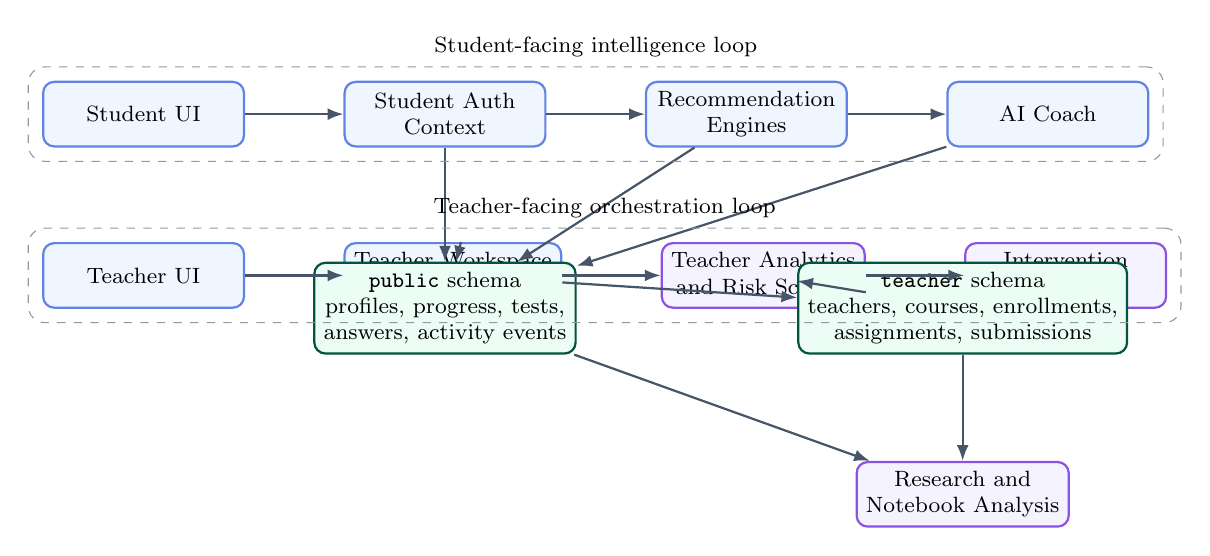
\begin{tikzpicture}[node distance=1.1cm and 1.25cm]
  \node[flow] (studentui) {Student UI};
  \node[flow, right=of studentui] (auth) {Student Auth\\Context};
  \node[flow, right=of auth] (reco) {Recommendation\\Engines};
  \node[flow, right=of reco] (coach) {AI Coach};

  \node[flow, below=1.2cm of studentui] (teacherui) {Teacher UI};
  \node[flow, right=of teacherui] (teachctx) {Teacher Workspace\\Aggregation};
  \node[insight, right=of teachctx] (analytics) {Teacher Analytics\\and Risk Scoring};
  \node[insight, right=of analytics] (insights) {Intervention\\Insights};

  \node[store, below=1.45cm of auth] (public) {\tech{public} schema\\profiles, progress, tests,\\answers, activity events};
  \node[store, right=2.8cm of public] (teacher) {\tech{teacher} schema\\teachers, courses, enrollments,\\assignments, submissions};

  \node[insight, below=1.35cm of teacher] (notebooks) {Research and\\Notebook Analysis};

  \draw[line] (studentui) -- (auth);
  \draw[line] (auth) -- (reco);
  \draw[line] (reco) -- (coach);
  \draw[line] (teacherui) -- (teachctx);
  \draw[line] (teachctx) -- (analytics);
  \draw[line] (analytics) -- (insights);

  \draw[line] (auth) -- (public);
  \draw[line] (reco) -- (public);
  \draw[line] (coach) -- (public);
  \draw[line] (teachctx) -- (public);
  \draw[line] (teachctx) -- (teacher);
  \draw[line] (analytics) -- (teacher);
  \draw[line] (public) -- (notebooks);
  \draw[line] (teacher) -- (notebooks);

  \node[group, fit=(studentui)(coach), label=above:{\footnotesize Student-facing intelligence loop}] {};
  \node[group, fit=(teacherui)(insights), label=above:{\footnotesize Teacher-facing orchestration loop}] {};
\end{tikzpicture}
\caption{High-level architecture of \project{}. The student portal, teacher portal, recommendation engines, and analytics layer all converge over a shared Supabase backbone.}
\end{figure*}

\subsection{Data Model}
The project uses a single Supabase project with two exposed schemas.

\textbf{Public schema:}
\begin{itemize}
  \item \tech{profiles}
  \item \tech{user\_progress}
  \item \tech{answered\_questions}
  \item \tech{test\_history}
  \item \tech{activity\_events}
\end{itemize}

\textbf{Teacher schema:}
\begin{itemize}
  \item \tech{teachers}
  \item \tech{courses}
  \item \tech{enrollments}
  \item \tech{assignments}
  \item \tech{submissions}
\end{itemize}

This schema split is one of the strongest architectural decisions in the repository. It preserves a clean distinction between student learning telemetry and teacher classroom operations while still allowing teacher analytics to read class-related student data through row-level security policies.

\section{Student Learning Flow}
\begin{itemize}
  \item Student signs in and the auth context restores local and cloud state.
  \item Profile, ELO, answered questions, subject scores, and enrolled courses are loaded.
  \item The learner joins one or more teacher classrooms using course codes.
  \item The learner chooses among full-paper, topic-wise, adaptive, or assignment flows.
  \item Results update ELO, subject progress, test history, and activity events.
  \item History review, dashboard analytics, and AI coach features reuse the same telemetry.
\end{itemize}

\section{Teacher Operational Flow}
\begin{itemize}
  \item Teacher signs in and the workspace is provisioned if necessary.
  \item Teacher creates courses and obtains unique join codes.
  \item Students enroll into courses.
  \item Teacher publishes assignments and monitors submissions.
  \item Teacher dashboard aggregates course, enrollment, submission, progress, and test history data.
  \item Risk scores, weak topics, and intervention suggestions guide follow-up action.
\end{itemize}

\section{Recommendation Systems Portfolio}
\begin{table*}[t]
\centering
\footnotesize
\begin{tabular}{>{\raggedright\arraybackslash}p{0.18\textwidth} >{\raggedright\arraybackslash}p{0.22\textwidth} >{\raggedright\arraybackslash}p{0.26\textwidth} >{\raggedright\arraybackslash}p{0.26\textwidth}}
\toprule
Engine & Primary purpose & Main inputs & Main outputs \\
\midrule
Adaptive next-best question engine & Choose the next practice question & subject, ELO, graph neighbors, session attempts, topic stats, reward signal & next question, reasons, target ELO, target difficulty, graph metadata \\
Remediation path engine & Recover after an incorrect answer & unresolved miss, graph hop limit, remediation history & easier or related follow-up path \\
Retry engine & Re-serve a missed question at the right time & remediation steps completed and remediation accuracy & retry of the original missed node \\
Rapid-guess review engine & Flag suspiciously fast correct attempts & time spent, question length, question type, question ELO & warning text and ELO penalty \\
AI coach engine & Generate study recommendations and coaching replies & weak topics, strong topics, recent tests, ELO, streak, focus area & summaries, plans, suggested follow-up actions \\
Teacher insight engine & Recommend classroom intervention & course summaries, student summaries, weak-topic frequency, completion rates & suggested assignments, focus students, top performers \\
GATE score prediction engine & Estimate future score range & ELO, completion, overall accuracy, consistency & min, expected, max score band and confidence \\
\bottomrule
\end{tabular}
\caption{Recommendation and decision-support systems embedded in the project.}
\end{table*}

\section{Adaptive Graph-Based Recommendation Engine}
\subsection{Design Objective}
The adaptive engine in \tech{src/lib/nextBestQuestionEngine.ts} does not simply sort questions by difficulty. It builds a recommendation graph over the question bank and navigates that graph using learner state.

\subsection{Core signals}
\begin{itemize}
  \item current student ELO
  \item recent correctness and reward signal
  \item momentum label: \tech{hot}, \tech{steady}, or \tech{cold}
  \item current topic and weakest recent topic
  \item already answered and already served question sets
  \item graph neighborhoods within configurable hop limits
  \item remediation progress for unresolved misses
\end{itemize}

\subsection{Graph construction}
Question nodes are linked using:
\begin{itemize}
  \item same subject and same topic relations
  \item difficulty transitions
  \item ELO closeness and progression fit
  \item type similarity and mark similarity
  \item subject anchors and topic anchors
\end{itemize}

Edge types are:
\begin{itemize}
  \item \tech{same-topic}
  \item \tech{subject-flow}
  \item \tech{subject-bridge}
\end{itemize}

\subsection{Target policy}
The engine computes a target ELO and target difficulty. It then searches either:

\begin{itemize}
  \item a remediation neighborhood around a missed question
  \item a neighbor neighborhood around the current question
  \item or a broader fallback pool
\end{itemize}

Candidates are scored with a combined heuristic and graph boost, then returned with natural-language reasons and graph metadata.

\begin{figure*}[t]
\centering
\begin{subfigure}[t]{0.48\textwidth}
\centering
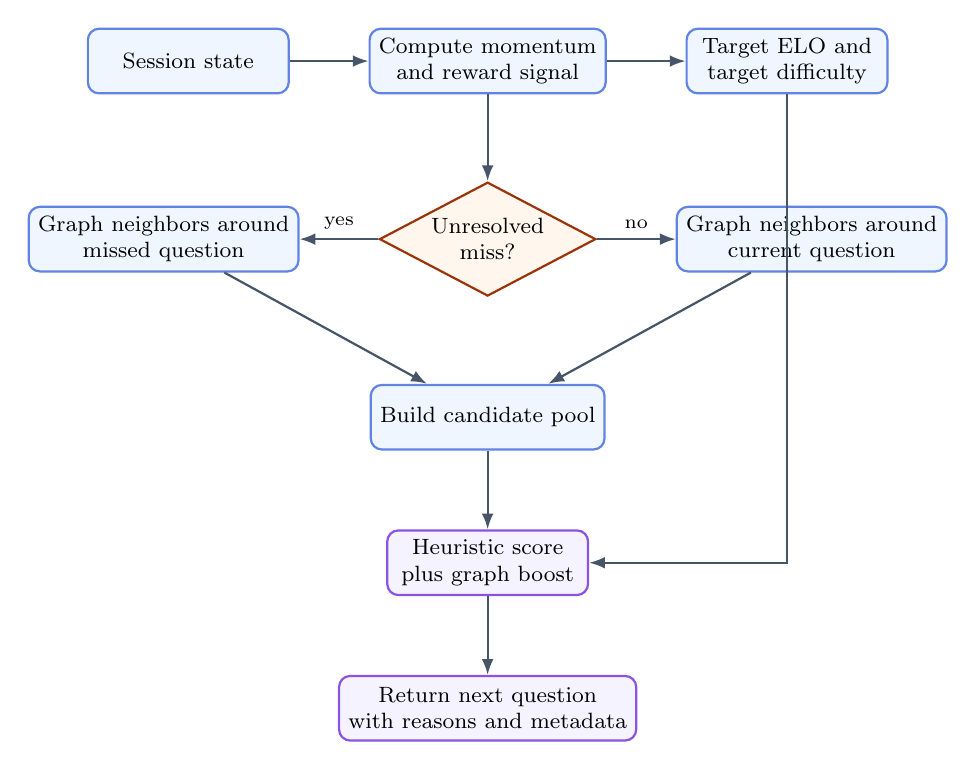
\begin{tikzpicture}[node distance=0.95cm and 1.0cm]
  \node[flow] (state) {Session state};
  \node[flow, right=of state] (momentum) {Compute momentum\\and reward signal};
  \node[flow, right=of momentum] (target) {Target ELO and\\target difficulty};

  \node[decision, below=1.1cm of momentum] (miss) {Unresolved\\miss?};
  \node[flow, left=1.0cm of miss] (remed) {Graph neighbors around\\missed question};
  \node[flow, right=1.0cm of miss] (curr) {Graph neighbors around\\current question};
  \node[flow, below=1.1cm of miss] (pool) {Build candidate pool};
  \node[insight, below=1.0cm of pool] (score) {Heuristic score\\plus graph boost};
  \node[insight, below=1.0cm of score] (out) {Return next question\\with reasons and metadata};

  \draw[line] (state) -- (momentum);
  \draw[line] (momentum) -- (target);
  \draw[line] (momentum) -- (miss);
  \draw[line] (miss) -- node[above, font=\scriptsize]{yes} (remed);
  \draw[line] (miss) -- node[above, font=\scriptsize]{no} (curr);
  \draw[line] (remed) -- (pool);
  \draw[line] (curr) -- (pool);
  \draw[line] (target) |- (score);
  \draw[line] (pool) -- (score);
  \draw[line] (score) -- (out);
\end{tikzpicture}
\caption{Adaptive recommendation flow.}
\end{subfigure}\hfill
\begin{subfigure}[t]{0.48\textwidth}
\centering
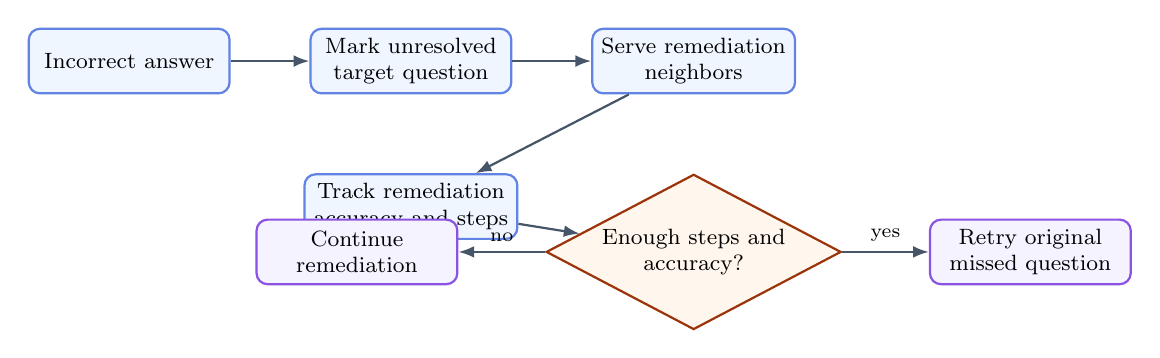
\begin{tikzpicture}[node distance=0.95cm and 1.0cm]
  \node[flow] (wrong) {Incorrect answer};
  \node[flow, right=of wrong] (targetq) {Mark unresolved\\target question};
  \node[flow, right=of targetq] (hops) {Serve remediation\\neighbors};
  \node[flow, below=1.0cm of targetq] (track) {Track remediation\\accuracy and steps};
  \node[decision, below=1.0cm of hops] (retry) {Enough steps and\\accuracy?};
  \node[insight, left=1.1cm of retry] (more) {Continue\\remediation};
  \node[insight, right=1.1cm of retry] (serve) {Retry original\\missed question};

  \draw[line] (wrong) -- (targetq);
  \draw[line] (targetq) -- (hops);
  \draw[line] (hops) -- (track);
  \draw[line] (track) -- (retry);
  \draw[line] (retry) -- node[above, font=\scriptsize]{no} (more);
  \draw[line] (retry) -- node[above, font=\scriptsize]{yes} (serve);
\end{tikzpicture}
\caption{Remediation and retry mechanism.}
\end{subfigure}
\caption{Side-by-side visualizations of the adaptive recommendation pipeline and its remediation logic.}
\end{figure*}

\section{Practice Review and ELO Control}
The practice review engine in \tech{src/lib/practiceReview.ts} estimates whether a correct answer may have been solved too quickly to count as full evidence of mastery. It computes a question-specific threshold from stem length, option length, and question type, then applies an ELO penalty if the solve time is below that threshold.

This design matters because the project avoids equating all correct answers with equal evidence. Fast but suspicious answers still contribute marks, but can produce reduced ELO gain and a stored warning in the review payload.

\section{AI Coach System}
\subsection{Hybrid execution model}
The AI coach in \tech{src/lib/aiCoach.ts} supports:
\begin{itemize}
  \item Gemini-backed structured JSON generation
  \item Ollama-backed generation through a managed proxy
  \item deterministic fallback logic with no external model dependency
\end{itemize}

\subsection{Coach intelligence}
The coach consumes:
\begin{itemize}
  \item ELO and current tier
  \item overall accuracy and total answered
  \item streak
  \item weak and strong subjects
  \item recent test results
  \item ongoing chat messages and focus area
\end{itemize}

Fallback logic is substantial rather than cosmetic. It can generate:
\begin{itemize}
  \item topic prioritization
  \item same-day study suggestions
  \item 3-day and 7-day plans
  \item mock-preparation advice
  \item revision allocation between weak and strong areas
\end{itemize}

\begin{figure}[t]
\centering
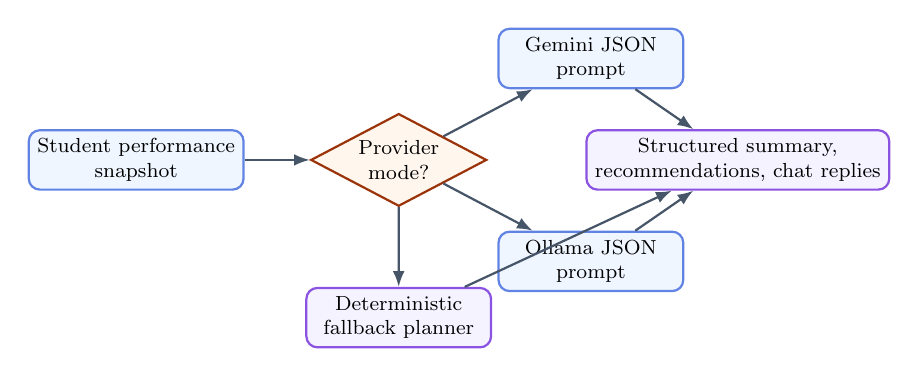
\begin{tikzpicture}[node distance=0.9cm and 0.9cm, scale=0.92, every node/.style={transform shape}]
  \node[flow] (input) {Student performance\\snapshot};
  \node[decision, right=of input] (prov) {Provider\\mode?};
  \node[flow, above right=0.65cm and 0.75cm of prov] (gem) {Gemini JSON\\prompt};
  \node[flow, below right=0.65cm and 0.75cm of prov] (oll) {Ollama JSON\\prompt};
  \node[insight, below=1.1cm of prov] (fb) {Deterministic\\fallback planner};
  \node[insight, right=1.35cm of prov] (parse) {Structured summary,\\recommendations, chat replies};

  \draw[line] (input) -- (prov);
  \draw[line] (prov) -- (gem);
  \draw[line] (prov) -- (oll);
  \draw[line] (prov) -- (fb);
  \draw[line] (gem) -- (parse);
  \draw[line] (oll) -- (parse);
  \draw[line] (fb) -- (parse);
\end{tikzpicture}
\caption{Hybrid AI coach architecture with LLM-backed and deterministic paths.}
\end{figure}

\section{Teacher Analytics and Intervention Intelligence}
\subsection{Teacher workspace aggregation}
The teacher workspace hook and classroom data layer aggregate:
\begin{itemize}
  \item teacher identity
  \item courses
  \item enrollments
  \item assignments
  \item submissions
  \item student profiles
  \item student progress rows
  \item student test history
  \item activity events
\end{itemize}

\subsection{Teacher summary outputs}
The analytics layer in \tech{src/lib/teacherAnalytics.ts} computes:
\begin{itemize}
  \item student summaries with ELO, accuracy, weak topics, assignment completion, and risk level
  \item course summaries with student count, assignment count, average accuracy, and completion rate
  \item recent activity items
  \item graph path sessions
  \item practice review sessions
  \item suggested assignments and focus students
\end{itemize}

\subsection{Risk scoring}
Risk is based on a blended score across:
\begin{itemize}
  \item overall student accuracy
  \item assignment completion rate
  \item ELO readiness
\end{itemize}

This translates raw telemetry into an actionable intervention queue for teachers.

\begin{figure}[t]
\centering
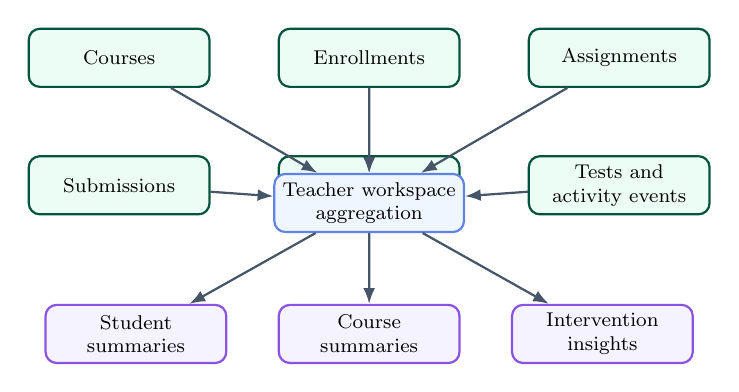
\begin{tikzpicture}[node distance=0.92cm and 0.95cm, scale=0.9, every node/.style={transform shape}]
  \node[store] (courses) {Courses};
  \node[store, right=of courses] (enroll) {Enrollments};
  \node[store, right=of enroll] (assign) {Assignments};
  \node[store, below=0.95cm of courses] (subs) {Submissions};
  \node[store, right=of subs] (prog) {User progress};
  \node[store, right=of prog] (tests) {Tests and\\activity events};

  \node[flow, below=1.2cm of enroll] (agg) {Teacher workspace\\aggregation};
  \node[insight, below left=1.0cm and 0.65cm of agg] (stud) {Student\\summaries};
  \node[insight, below=1.0cm of agg] (course) {Course\\summaries};
  \node[insight, below right=1.0cm and 0.65cm of agg] (intervene) {Intervention\\insights};

  \draw[line] (courses) -- (agg);
  \draw[line] (enroll) -- (agg);
  \draw[line] (assign) -- (agg);
  \draw[line] (subs) -- (agg);
  \draw[line] (prog) -- (agg);
  \draw[line] (tests) -- (agg);
  \draw[line] (agg) -- (stud);
  \draw[line] (agg) -- (course);
  \draw[line] (agg) -- (intervene);
\end{tikzpicture}
\caption{Teacher analytics pipeline from classroom data to actionable insight.}
\end{figure}

\section{GATE Score Prediction}
The score prediction module in \tech{src/components/GateScorePrediction.tsx} estimates a score band using a weighted combination of:

\begin{itemize}
  \item overall accuracy
  \item normalized ELO
  \item subject consistency
  \item improvement factor
\end{itemize}

The current implementation unlocks the predictor only after all of the following:
\begin{itemize}
  \item ELO $\geq 2500$
  \item full mock completion $\geq 70\%$
  \item topic-wise completion $\geq 70\%$
  \item adaptive completion $\geq 70\%$
\end{itemize}

The main formula is conceptually:
\[
\text{PredictedScoreBasis} =
0.4(\text{Accuracy}) +
0.3(\text{ELO}_{norm}) +
0.2(\text{Consistency}) +
0.1(\text{Improvement})
\]

The predictor then converts this basis into:
\begin{itemize}
  \item minimum expected score
  \item expected score
  \item maximum expected score
  \item confidence
  \item recommendation text
\end{itemize}

\section{Telemetry, Sync, and Persistence}
One of the most important engineering features of the project is that it records both state and events.

\subsection{State persistence}
The student auth context persists:
\begin{itemize}
  \item ELO
  \item answered question IDs
  \item subject scores
  \item profiles
  \item test history
\end{itemize}

\subsection{Event persistence}
The \tech{activity\_events} table stores:
\begin{itemize}
  \item sign-up and sign-in activity
  \item question answers
  \item test completion
  \item graph path completion
  \item practice session completion
  \item course joins and leaves
  \item teacher course and assignment operations
\end{itemize}

\subsection{Why this is valuable}
This event stream enables:
\begin{itemize}
  \item teacher recent activity views
  \item graph path reconstruction
  \item practice review sessions
  \item notebook-based longitudinal analytics
  \item better explainability for recommendation outcomes
\end{itemize}

\begin{figure*}[t]
\centering
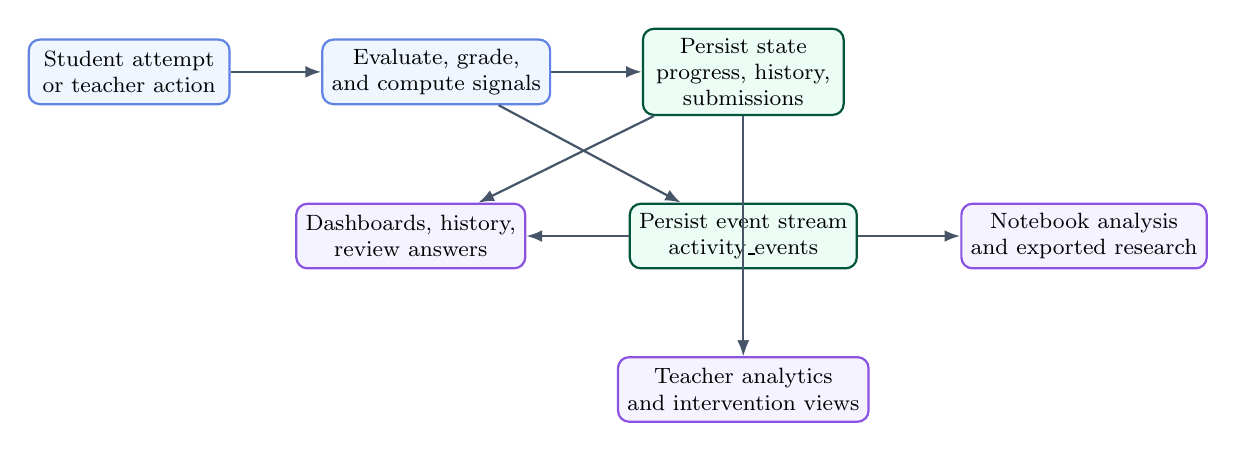
\begin{tikzpicture}[node distance=1.0cm and 1.15cm]
  \node[flow] (attempt) {Student attempt\\or teacher action};
  \node[flow, right=of attempt] (eval) {Evaluate, grade,\\and compute signals};
  \node[store, right=of eval] (state) {Persist state\\progress, history,\\submissions};
  \node[store, below=1.1cm of state] (events) {Persist event stream\\activity\_events};
  \node[insight, left=1.3cm of events] (dash) {Dashboards, history,\\review answers};
  \node[insight, below=1.1cm of events] (teacherdash) {Teacher analytics\\and intervention views};
  \node[insight, right=1.3cm of events] (nb) {Notebook analysis\\and exported research};

  \draw[line] (attempt) -- (eval);
  \draw[line] (eval) -- (state);
  \draw[line] (eval) -- (events);
  \draw[line] (state) -- (dash);
  \draw[line] (events) -- (dash);
  \draw[line] (events) -- (teacherdash);
  \draw[line] (state) -- (teacherdash);
  \draw[line] (events) -- (nb);
\end{tikzpicture}
\caption{Telemetry and persistence flow from user actions to dashboards, analytics, and research assets.}
\end{figure*}

\section{History Review and Explainability}
The recent review enhancement adds a \tech{review\_payload} to test history. This allows the platform to reconstruct past sessions with:

\begin{itemize}
  \item question IDs
  \item submitted answers
  \item optional question review metadata
  \item timing warnings
  \item explanation replay
\end{itemize}

This is a high-value feature because it upgrades history from static score summaries to replayable learning evidence.

\section{Research Assets and Visual Analytics}
The repository includes analysis tooling beyond the live product:

\begin{itemize}
  \item \tech{tools/generate\_gate\_da\_question\_graph\_notebook.py}
  \item \tech{tools/generate\_gate\_da\_student\_progress\_notebook.py}
  \item a teacher dashboard mockup generator
\end{itemize}

These notebooks support graph export, performance trend analysis, and exploratory analytics over the same data model used by the app.

\section{Testing and Validation}
The project contains direct test coverage for the adaptive engine. Current unit tests validate:

\begin{itemize}
  \item easier same-topic follow-up after a miss
  \item remediation path generation
  \item harder follow-up after a correct answer
  \item retrying a missed question after sufficient remediation
  \item exclusion of previously answered or already served questions
\end{itemize}

This is especially important because recommendation logic is the intellectual core of the platform.

\section{Strengths}
\begin{itemize}
  \item clean role separation between student and teacher experiences
  \item strong use of Supabase schemas and row-level security
  \item explainable recommendation outputs with metadata and reasons
  \item event-driven observability through \tech{activity\_events}
  \item hybrid AI architecture with deterministic fallback
  \item replayable history and review answers
  \item teacher-facing intervention support rather than passive reporting
  \item notebook-backed research layer that complements the UI
\end{itemize}

\section{Limitations and Future Enhancements}
\begin{itemize}
  \item formal experiment tracking for recommendation-policy comparisons is not yet first-class
  \item more longitudinal in-app analytics could be surfaced directly from the event stream
  \item score prediction history could be persisted for trend analysis
  \item spaced repetition and prerequisite graphs could extend the recommendation engine further
  \item recommendation quality metrics and A/B experimentation could be added for academic evaluation
\end{itemize}

\section{Conclusion}
\project{} should be presented as an explainable, classroom-aware, multi-engine recommendation platform for GATE DA preparation. Its most valuable innovation is not any single page, but the way student performance, graph structure, event telemetry, teacher analytics, and AI assistance are unified into one coherent educational system.

In summary, the project integrates:
\begin{itemize}
  \item product engineering
  \item recommender-system design
  \item adaptive remediation logic
  \item educational analytics
  \item teacher intervention intelligence
  \item hybrid AI-assisted guidance
\end{itemize}

That combination makes it well-suited for an advanced project report, viva, research presentation, or technical portfolio submission.

\end{document}
